\section{Proces regulacji ciśnienia i prędkości przepływu w układzie hydraulicznym}
Proces polega na wykorzystaniu falownika do regulacji pracy pompy, odpowiedzialnej za prędkość przepływu oraz ciśnienie wody znajdującej się w układzie hydraulicznym.Sterownik PLC wysyła poprzez sieć ProfiBus wartość częstotliwości którą falownik wyzerowuje prace pompy, ciśnienie jest także regulowane za pomocą zaworów znajdujących się w układzie hydraulicznym.Do sterownika powraca wartość ciśnienia zmierzonego przy pomocy czujnika analogowego oraz wartości przepływu liczonego poprzez czujnik impulsowy.Dane z pomiarów są zapisywane i wyświetlane na panelu operatorskim umożliwiając dobór parametrów operatorowi.
\newpage
\subsection{Układ hydrauliczny}
Układ na którym opiera się proces został znajduję się na zdjęciu poniżej.
\begin{figure}[h]
\centering
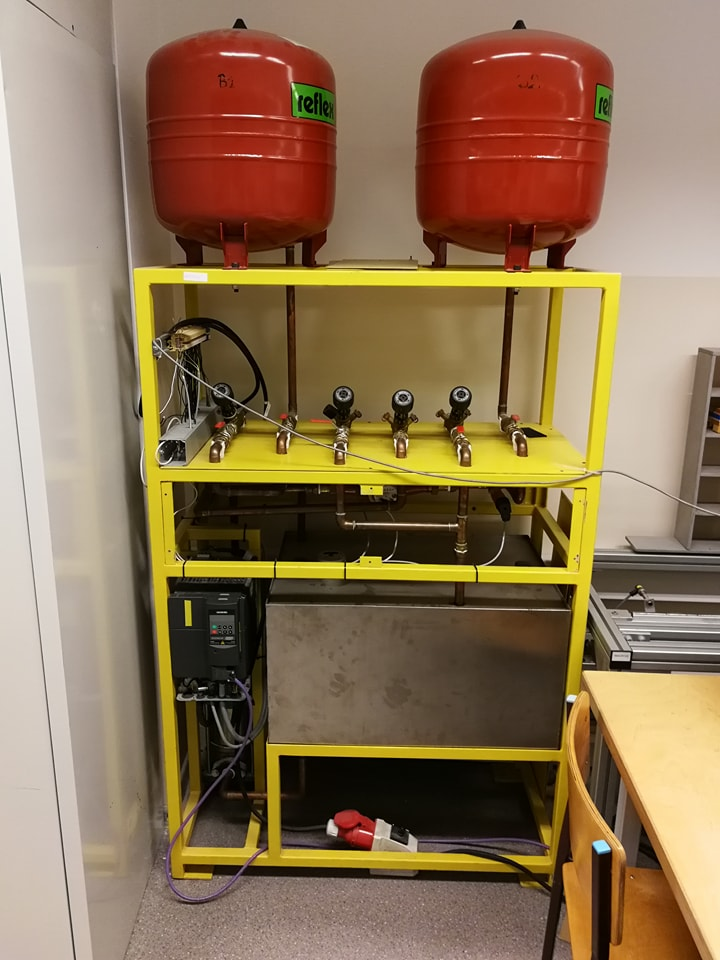
\includegraphics[scale=0.3]{Zdjecia/Stanowiska/4_Pompa/uklad_h.jpg}
\caption{Układ hydrauliczny}
\end{figure}

Układ składa się z zbiornika przelewowego umieszczonego najniżej.Woda za pomocą pompy jest tłoczona w układ rur, które dzielą się na dwa podukłady.Każdy podukład rur kieruje wodę do zbiornika grawitacyjnego oraz z powrotem do zbiornika przelewowego. Układ wyposażony jest w pięć zaworów prostych oraz trzy zawory do precyzyjnej regulacji przepływu.Pierwszy zawór prosty odpowiada za przebieg wody z zbiornika przelewowego do układu.Pozostałe pary zaworów, precyzyjny i prosty, znajdują się  w każdym z podukładów na rurze prowadzącej z powrotnym obiegiem do zbiornika przelewowego,poza tym zawór prosty na połączeniu do każdego zbiornika grawitacyjnego.Ostatni zawór precyzyjny znajduje się na złączeniu podukładów.
\newpage
\subsection{Czujnik MBS 33 z separatorem SD-2 oraz przepływomierz}
\fontseries{b}\selectfont
Czujnik ciśnienia MBS 33\\
\fontseries{m}\selectfont
Do pomiarów wartości ciśnienia wykorzystany został czujnik ciśnienia MBS33.

\begin{figure}[h]
\centering
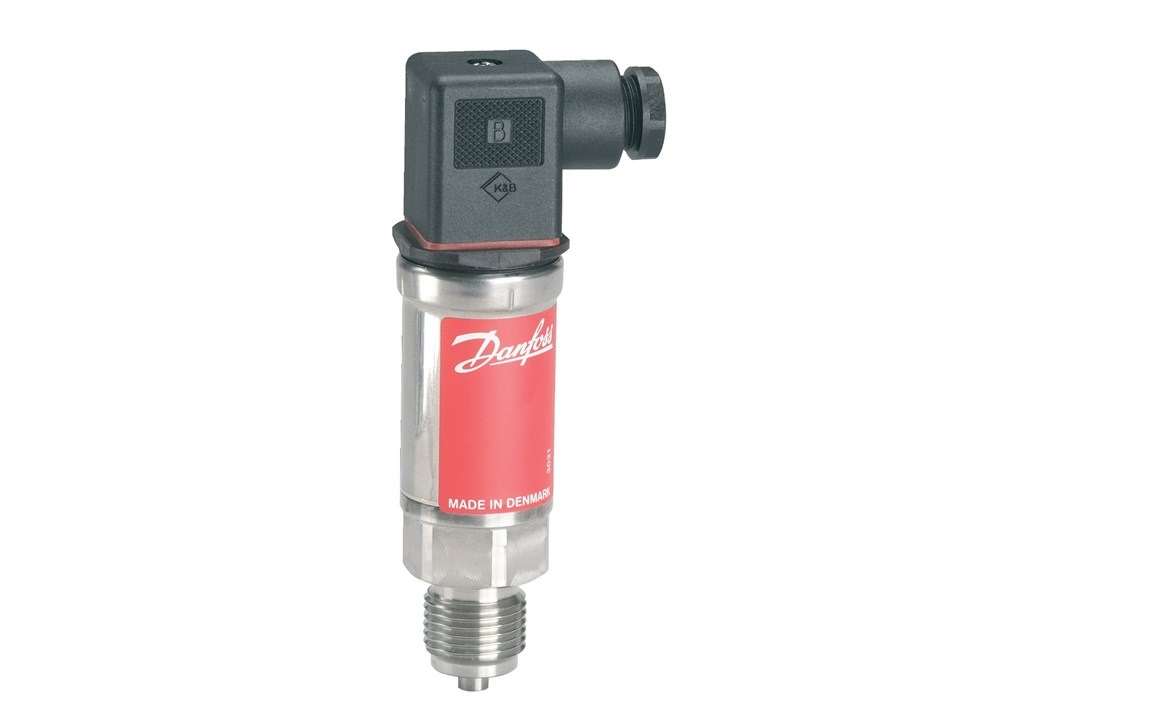
\includegraphics[scale=0.45]{Zdjecia/Stanowiska/4_Pompa/MBS_33.jpg}
\caption{Czujnik ciśnienia MBS 33}
\end{figure}

Przetwornik ciśnienia MBS 33 posiada sygnał wyjściowy o zakresie  4 - 20 mA, który przekłada się na pomiar względnego lub absolutnego w zakres od 0 do 6 bar.Czujnik wykazuje bardzo dobra odporność na wibracje oraz wytrzymałą budowę co pozwala na pracę w trudnych warunkach, zakres temperatury w której może pracować to od -40 do 85° C.
\cite{diduce:MBS33}.\\

\fontseries{b}\selectfont
Separator obwodów analogowych S2-D
\fontseries{m}\selectfont

W celu przekazania sygnału 0-20mA na moduł we/wy analogowych SM334 wykorzystujemy separator obwodów analogowych S2-D.
Jest to niezbędne ponieważ moduł SM334 nie pozwala na odczyt wartości analogowych będących wartościami natężenia.

\begin{figure}[h]
\centering
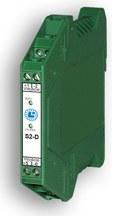
\includegraphics[scale=1.3]{Zdjecia/Stanowiska/4_Pompa/SD-2.jpg}
\caption{Separator obwodów analogowych S2-D}
\end{figure}
\newpage
Separator S2-D oddziela galwanicznie obwody wejściowego pomiarowego od pomiarowego obwodu wyjściowego.Jest  zasilane ze źródła napięcia stałego 24Vdc.Pozwala na zmniejszenie wpływu zakłóceń emitujących wpływ różnic potencjałów mas oraz pozwala odseparować różne standardy sygnałów 0-5mA, 0-20mA, 4-20mA, 0-5V, 0-10V, 1-5V.
\\Wykorzystane przez nas zostało ustawienie: wejście 0...20mA, wyjście 0...10V. Separator zostawał zasilony za pomocą zasilacza 24V.
\cite{diduce:SD-2}.\\

\fontseries{b}\selectfont
Przepływomierz
\fontseries{m}\selectfont

Wykorzystany przepływomierz podłączony jest do modułu SM321 pozwalającego na odczyt sygnałów cyfrowych.Wysyła on impuls co 0.1l przepuszczonej wody.Został zasilony (Sprawdzić czym!!!!)
\subsection{Moduły SM321 i SM 334}
\fontseries{b}\selectfont
Moduł wejść cyfrowych SM321
\fontseries{m}\selectfont

Moduł SM321 pozwala na odczyt sygnałów cyfrowych.W projekcie został użyty do odczytu sygnału z przepływomierza.

\begin{figure}[h]
\centering
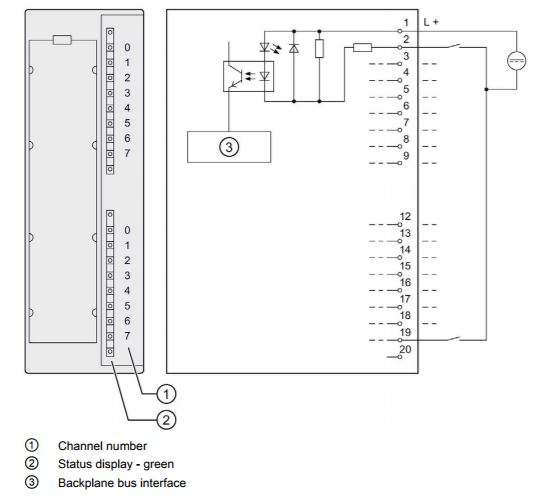
\includegraphics[scale=0.8]{Zdjecia/Stanowiska/4_Pompa/SM321_sch.jpg}
\caption{Schemat modułu wejść cyfrowych SM321}
\end{figure}

Moduł SM321 posiada 16 wejść cyfrowych o napięciu znamionowym 24V.
\cite{diduce:S7-300}.\\
\newpage
\fontseries{b}\selectfont
Moduł SM324
\fontseries{m}\selectfont

Zastosowany w tym procesie został również moduł wejść/wyjść analogowych SM334 identyczny jak w powyżej opisanych procesach. Został on wykorzystany do odbioru sygnału z wartością pomierzonego ciśnienia.
\subsection{Falownik i Pompa}
\fontseries{b}\selectfont
Przekształtnik częstotliwości Micromaster 440
\fontseries{m}\selectfont

Za pracę pompy odpowiedzialny jest przekształtnik częstotliwości Micromaster 440. Jest przeznaczony do
regulacji prędkości obrotowej silników trójfazowych. 
\begin{figure}[h]
\centering
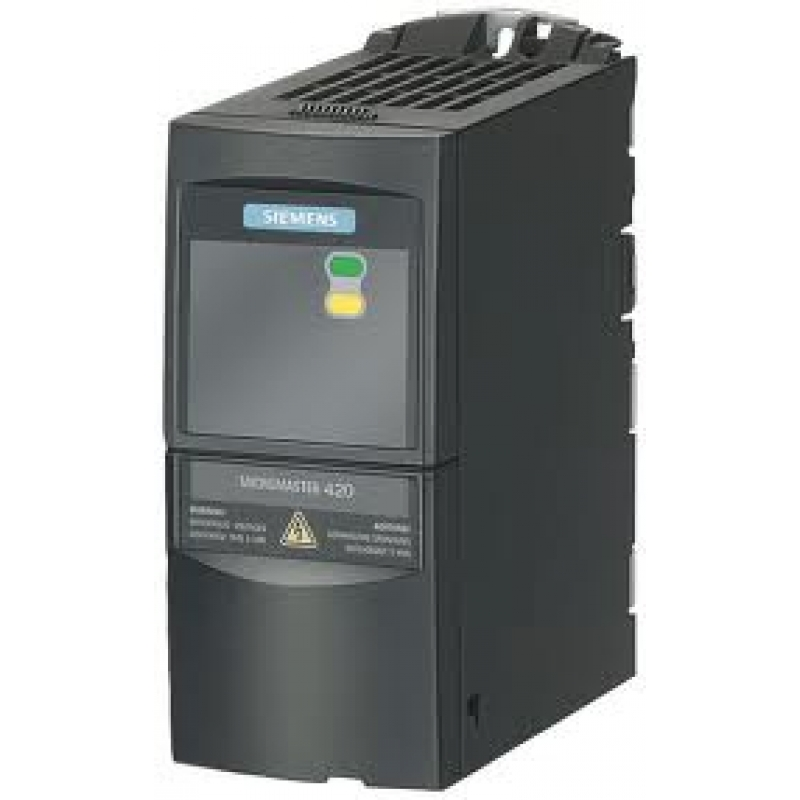
\includegraphics[scale=0.3]{Zdjecia/Stanowiska/4_Pompa/Micromaster440.jpg}
\caption{Micromaster 440 wyposażony w moduł komunikacyjny sieci ProfiBus oraz panel BOP}
\end{figure}

Falownik tego modelu posiada wysokie częstotliwości pulsowania, które zapewniają cichą prace silnika,szeroki wybór parametrów umożliwiający dostosowanie konfiguracji do projektu oraz budowę modułową.W tym przypadku został wykorzystany panel BOP czyli podstawowy panel operatorski,który pozwala na zmianę parametrów.Dodany został również moduł komunikacji ProfiBus zapewniający komunikacje falownika z sterownikiem PLC.
\cite{diduce:MICROMASTER}.\\

\fontseries{b}\selectfont
Pompa
\fontseries{m}\selectfont 

Pompa wykorzystana w procesie została wyprodukowana przez firmę Wilo AG model 44263 typ MVI107 1/16/E/3-400-50-2.Ma możliwość pracy do 16 bar przy temperaturze maksymalnej 120°C.
\subsection{Komunikacja PLC-Micromaster z użyciem sieci ProfiBus}